{\color{red}
\myparagraph{Le nano-ordinateur}
\label{jetson_nano_lego}
\begin{figure}[H]
    \centering
    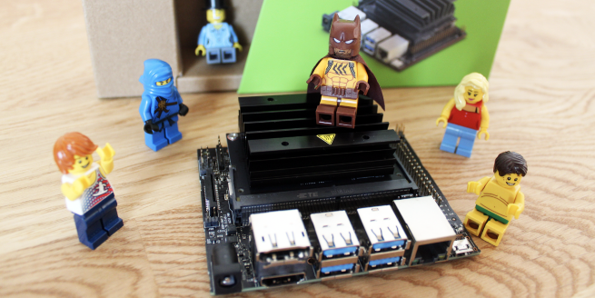
\includegraphics[width=1.0\textwidth]{jetson_nano_lego}
    \caption{Photo de la carte mère Jetson Nano de NVIDIA, représenté avec des légos pour démontrer sa petitesse}
    \label{fig:jetson_nano_lego}
\end{figure}

\par L'objet d'étude de cet essai est un nano-ordinateur. Un nano-ordinateur est un ordinateur miniaturisé en taille, mais aussi limité en capacité. Il existe différents fabricants et modèles, de caractéristiques techniques variées, pour répondre à différents besoins. Le dernier né est le modèle "Jetson nano" du fabricant "NVIDIA", disponible depuis juin 2019 au prix très abordable de 99\$US. La compagnie NVIDIA a conçu ce matériel spécialement pour différentes applications d'inférence de modèles d'apprentissage profond sur une plateforme mobile (drone) ou proche des données ("edge" en anglais). Ce modèle a été choisi afin de répondre à l'intérêt que suscitent ses capacités et ses limites. 
\todo{TODO}

\myparagraph{Logiciels}
\todo{TODO}
\par De même que pour les périphériques, les logiciels qui seront utilisés seront résumés dans un tableau, où il sera indiqué leur nom, le type de licence, leur version, leurs avantages et limitations, comme pour le système d'exploitation, l'environnement de développement pour l'apprentissage profond, l'inférence, les logiciels de traitements vidéos et d'images. 
\begin{itemize}
   \item Présentation du SDK qui sera installé (JetPack, Linux for Tegra L4T, Cuda CuDnn, TensorRT);
   \item Présentation des frameworks d’apprentissage profond qui vont être utilisés (PyTorch, torchvision);
   \item Présentation des librairies pour d'inférence (TensorRT, onnx);
\end{itemize}
}